\begin{center}
{\Large\bfseries 前言}
\end{center}

\qquad 最近整理了一份~\LaTeX{} 绘图笔记,内容主要侧重于绘制中学学习教材上用到的大部分图,对于~\LaTeX{} 绘图的入门,初学者可以进入~\LaTeX{} 工作室官网寻找一些 TikZ 的绘图入门,其中有~\href{https://www.latexstudio.net/index/details/index/mid/940.html}{\textcolor{orange}{TikZ 绘图入门基础}}、\href{https://www.latexstudio.net/index/details/index/mid/878.html} {\textcolor{blue}{TikZ 学习笔记}}、\href{https://www.latexstudio.net/index/details/index/mid/949.html} {\textcolor{cyan}{TikZ/PGF manual}} 以及~TikZ 绘图宏包的学习手册。相关的资源可以关注公众号动态,以及工作室官方网站。

\begin{multicols}{2}
\centerline{
\includegraphics[scale=0.15]{fig2}}
\centerline{
\includegraphics[scale=0.1]{fig1}}
\end{multicols}

{\centering
\begin{tikzpicture}
  \begin{scope}[color=cyan]

  \node[minimum size=15cm](current page1){};
  \node[scale=0.5,anchor=north west] at (current page1.north west)
  {\pgfornament[width=7cm]{35}};
  \node[scale=0.5,anchor=west,rotate=45] at (current page1.west)
  {\pgfornament[width=7cm]{35}};
  \node[scale=0.5,anchor=north east] at (current page1.north east)
  {\pgfornament[width=7cm]{36}};
  \node[scale=0.5,anchor=east,rotate=-45] at (current page1.east)
  {\pgfornament[width=7cm]{36}};
  \node[scale=0.5,anchor=south west] at (current page1.south west)
  {\pgfornament[width=7cm,symmetry=h]{35}};
  \node[scale=0.5,anchor=south,rotate=45] at (current page1.south)
  {\pgfornament[width=7cm,symmetry=h]{35}};
  \node[scale=0.5,anchor=south east] at (current page1.south east)
  {\pgfornament[width=7cm,symmetry=h]{36}};
  \node[scale=0.5,anchor=south,rotate=-45] at (current page1.south)
  {\pgfornament[width=7cm,symmetry=h]{36}};
  \node[scale=20,green!45!black,cloud,cloud puffs=14,draw=blue,fill=pink]at(current page1.center){\scalebox{0.1}{~~~~~~~~}};
  \end{scope}

  \node[scale=1.45]at (0,0.7){
  \begin{tikzpicture}
 \foreach \i in {0,0.01,...,2}
     \draw[draw=white,rotate=-95,thick]($(0,0) !1! \i*180:(3,2)$)--($(1,0) !1! \i*360:(2,2)$);
     \begin{scope}
     \node[scale=2,green!45!black,rotate=55]at(-2.3,1.2){2};
     \node[scale=2,green!45!black,rotate=45]at(-2,1.5){0};
     \node[scale=2,green!45!black,rotate=40]at(-1.7,1.8){2};
     \node[scale=2,green!45!black,rotate=25]at(-1.3,2){0};
     \node[scale=2,green!45!black,rotate=-55]at(2.3,1.2){1};
     \node[scale=2,green!45!black,rotate=-45]at(2,1.5){2};
     \node[scale=2,green!45!black,rotate=-40]at(1.7,1.8){0};
     \node[scale=2,green!45!black,rotate=-25]at(1.3,2){2};
     \node[scale=2,green!45!black,rotate=0]at(0,4){Happy};
     \node[scale=1.5,green!45!black,rotate=0]at(0,2.8){New Year};
  \end{scope}
         \end{tikzpicture}};

  \end{tikzpicture}
}
\vspace{-1cm}
\textcolor{orange}{\dotfill}~\textit{全世界在等我飞更高~~你却心疼我受伤翅膀}
\thispagestyle{empty}
\clearpage
\thispagestyle{empty}
\begin{center}
{\Large\bfseries 分享}
\end{center}

\qquad 在学习~TikZ 绘图过程中,偶尔看见别人用~Blender 结合 Python 绘制心线图的动画视频,于是常识了用~\LaTeX 中 TikZ 宏包去实现,最后绘制出来了,这里进行代码分享!

首先是心线图的绘制:

%\noindent
%\textcolor{orange}{\dotfill}\\
\vspace{3pt}
\begin{minipage}[c]{0.51\textwidth}
  \centering
  \begin{lstlisting}[gobble=8]
        \begin{tikzpicture}
         \foreach \i in {0,0.02,...,2} % foreach 循环语句
           \draw
                [
                 draw=cyan,  % 绘制线条颜色
                 rotate=-124 % 旋转角度
                ]
                ($(0,0) !1! \i*180:
                (3,2)$)--($(0,0) !1! \i*360:(3,2)$);
                % 在圆上标记100个等分点,依次从0标记到99,每个点连接标记是它2倍
                %的点,最后形成心线!
        \end{tikzpicture}
  \end{lstlisting}
  \vspace{2pt}
\end{minipage}
\hfil
\begin{minipage}[c]{0.45\textwidth}
  \centering
  \vspace{3pt}
  \begin{tikzpicture}[scale=0.6]
  \draw[blue](-6.5,-4)--(-6.5,4);
  \draw[dashed](-6,-4) rectangle (6,4);
  \foreach \i in {0,0.02,...,2}
  \draw[draw=cyan,rotate=-124]($(0,0) !1! \i*180:(3,2)$)--($(0,0) !1! \i*360:(3,2)$);
\end{tikzpicture}
\vspace{2pt}
\end{minipage}
%\noindent
%\textcolor{orange}{\rule{\textwidth}{0.6pt}}


类似地,我们连接的点变成3倍、4倍甚至n倍,以及小数点倍会是怎样的感觉呢,下面来看看:

\vspace{3pt}
\begin{minipage}[c]{0.51\textwidth}
  \centering
  \begin{lstlisting}[gobble=8]
        \begin{tikzpicture}
         \foreach \i in {0,0.02,...,2} % foreach 循环语句
           \draw
                [
                 draw=cyan,  % 绘制线条颜色
                 rotate=-124 % 旋转角度
                ]
                ($(0,0) !1! \i*180:(3,2)$)--($(0,0) !1! \i*540:(3,2)$);
                % 在圆上标记100个等分点,依次从0标记到99,每个点连接标记是它3倍
                %的点,最后形成心线!
        \end{tikzpicture}
  \end{lstlisting}
  \vspace{2pt}
\end{minipage}
\hfil
\begin{minipage}[c]{0.45\textwidth}
  \centering
  \vspace{3pt}
  \begin{tikzpicture}[scale=0.6]
  \draw[orange](-6.5,-4)--(-6.5,4);
  \draw[draw=blue,dashed](-6,-4) rectangle (6,4);
  \foreach \i in {0,0.02,...,2}
  \draw[draw=blue,rotate=-124]($(0,0) !1! \i*180:(3,2)$)--($(0,0) !1! \i*540:(3,2)$);
\end{tikzpicture}
\vspace{2pt}
\end{minipage}

连接点数是其标记点数~4 倍的时候是这样的,图像如下:

\vspace{3pt}
\begin{minipage}[c]{0.51\textwidth}
  \centering
  \begin{lstlisting}[gobble=8]
        \begin{tikzpicture}
         \foreach \i in {0,0.02,...,2} % foreach 循环语句
           \draw
                [
                 draw=cyan,  % 绘制线条颜色
                 rotate=-124 % 旋转角度
                ]
                ($(0,0) !1! \i*180:(3,2)$)--($(0,0) !1! \i*720:(3,2)$);
                % 在圆上标记100个等分点,依次从0标记到99,每个点连接标记是它3倍
                %的点,最后形成心线!
        \end{tikzpicture}
  \end{lstlisting}
  \vspace{2pt}
\end{minipage}
\hfil
\begin{minipage}[c]{0.45\textwidth}
  \centering
  \vspace{3pt}
  \begin{tikzpicture}[scale=0.6]
  \draw[Orange](-6.5,-4)--(-6.5,4);
  \draw[draw=Blue,dashed](-6,-4) rectangle (6,4);
  \foreach \i in {0,0.02,...,2}
  \draw[draw=orange,rotate=-124]($(0,0) !1! \i*180:(3,2)$)--($(0,0) !1! \i*720:(3,2)$);
\end{tikzpicture}
\vspace{2pt}
\end{minipage}

下列代码运行生成多页PDF格式文档,运用宏包~animate 制作动画:


\begin{lstlisting}[gobble=8]
        \documentclass{ctexart}
        \usepackage{ctex}
        \usepackage{amsmath}
        \usepackage{tikz}
        \usetikzlibrary{calc}\tikzset{>=latex}
        \usepackage{pgfplots}
        \usepackage[active,tightpage]{preview}
        \PreviewEnvironment{tikzpicture}
        \setlength\PreviewBorder{0pt}
        \definecolor{myback}{RGB}{53,64,89}
        \definecolor{mycolor}{RGB}{51,51,51}
        \definecolor{Orange}{RGB}{102,51,0}
        \definecolor{Green}{RGB}{0,102,51}
        \definecolor{Blue}{RGB}{15,107,108}
        \definecolor{Yellow}{RGB}{153,151,51}
        \begin{document}
                  \foreach \N in {0.1,0.0995,...,0}{
                          \begin{tikzpicture}
                            \draw[fill=myback](-6,-4) rectangle (6,5);
                            \draw[fill=myback](-6,-4) rectangle (6,4);
                                \foreach \i in {0,\N,...,2}
                            \draw[draw=orange!60!yellow,rotate=-124]($(0,0) !1! \i*180:(3,2)$)--($(0,0) !1! \i*400:(2,2)$);
                          \end{tikzpicture}}
        \end{document}
\end{lstlisting}
\thispagestyle{empty}
\vspace{3pt}
\begin{minipage}[c]{0.51\textwidth}
  \centering
  \begin{lstlisting}[gobble=8]
        \begin{tikzpicture}
         \foreach \i in {0,0.02,...,2} % foreach 循环语句
           \draw
                [
                 draw=cyan,  % 绘制线条颜色
                 rotate=-124 % 旋转角度
                ]
                ($(0,0) !1! \i*180:(3,2)$)--($(0,0) !1! \i*900:(3,2)$);
                % 在圆上标记100个等分点,依次从0标记到99,每个点连接标记是它3倍
                %的点,最后形成心线!
        \end{tikzpicture}
  \end{lstlisting}
  \vspace{2pt}
\end{minipage}
\hfil
\begin{minipage}[c]{0.45\textwidth}
  \centering
  \vspace{3pt}
  \begin{tikzpicture}[scale=0.6]
  \draw[Orange](-6.5,-4)--(-6.5,4);
  \draw[draw=Blue,dashed](-6,-4) rectangle (6,4);
  \foreach \i in {0,0.02,...,2}
  \draw[draw=Blue,rotate=-124]($(0,0) !1! \i*180:(3,2)$)--($(0,0) !1! \i*900:(3,2)$);
\end{tikzpicture}
\vspace{2pt}
\end{minipage}


\vspace{3pt}
\begin{minipage}[c]{0.51\textwidth}
  \centering
  \begin{lstlisting}[gobble=8]
        \begin{tikzpicture}
         \foreach \i in {0,0.02,...,2} % foreach 循环语句
           \draw
                [
                 draw=cyan,  % 绘制线条颜色
                 rotate=-124 % 旋转角度
                ]
                ($(0,0) !1! \i*180:(3,2)$)--($(0,0) !1! \i*1800:(3,2)$);
                % 在圆上标记100个等分点,依次从0标记到99,每个点连接标记是它3倍
                %的点,最后形成心线!
        \end{tikzpicture}
  \end{lstlisting}
  \vspace{2pt}
\end{minipage}
\hfil
\begin{minipage}[c]{0.45\textwidth}
  \centering
  \vspace{3pt}
  \begin{tikzpicture}[scale=0.6]
  \draw[Orange](-6.5,-4)--(-6.5,4);
  \draw[draw=Blue,dashed,fill=pink](-6,-4) rectangle (6,4);
  \foreach \i in {0,0.02,...,2}
  \draw[draw=white,rotate=-124,thick]($(0,0) !1! \i*180:(3,2)$)--($(0,0) !1! \i*1800:(3,2)$);
\end{tikzpicture}
\vspace{2pt}
\end{minipage}

\vspace{-3pt}
\begin{minipage}[c]{0.51\textwidth}
  \centering
  \begin{lstlisting}[gobble=8]
        \begin{tikzpicture}
         \foreach \i in {0,0.02,...,2} % foreach 循环语句
           \draw
                [
                 draw=cyan,  % 绘制线条颜色
                 rotate=-124 % 旋转角度
                ]
                ($(0,0) !1! \i*180:(3,2)$)--($(0,0) !1! \i*620:(3,2)$);
                % 在圆上标记100个等分点,依次从0标记到99,每个点连接标记是它3倍
                %的点,最后形成心线!
        \end{tikzpicture}
  \end{lstlisting}
  \vspace{2pt}
\end{minipage}
\hfil
\begin{minipage}[c]{0.45\textwidth}
  \centering
  \vspace{3pt}
  \begin{tikzpicture}[scale=0.6]
  \draw[Orange](-6.5,-4)--(-6.5,4);
  \draw[draw=Blue,dashed,fill=green!15!white](-6,-4) rectangle (6,4);
  \foreach \i in {0,0.02,...,2}
  \draw[draw=yellow!80!red!20!green,rotate=-124]($(0,0) !1! \i*180:(3,2)$)--($(0,0) !1! \i*620:(3,2)$);
\end{tikzpicture}
\vspace{2pt}
\end{minipage}


\vspace{3pt}
\begin{minipage}[c]{0.51\textwidth}
  \centering
  \begin{lstlisting}[gobble=8]
        \begin{tikzpicture}
          \foreach \i in {0,0.02,...,2}
          \draw[
          draw=orange!80!red!20!green,
          rotate=-124
          ]($(0,0)
          !1! \i*180:(3,2)$)--($(0,0) !1!
          \i*7120:(3,2)$);
        \end{tikzpicture}
  \end{lstlisting}
  \vspace{2pt}
\end{minipage}
\hfil
\begin{minipage}[c]{0.45\textwidth}
  \centering
  \vspace{3pt}
  \begin{tikzpicture}[scale=0.6]
  \draw[Orange](-6.5,-4)--(-6.5,4);
  \draw[draw=Blue,dashed,fill=pink!15!white](-6,-4) rectangle (6,4);
  \foreach \i in {0,0.02,...,2}
  \draw[draw=orange!80!red!20!green,rotate=-124]($(0,0) !1! \i*180:(3,2)$)--($(0,0) !1! \i*7120:(3,2)$);
\end{tikzpicture}
\vspace{2pt}
\end{minipage}

\thispagestyle{empty}


\begin{tikzpicture}
    \node at (0,2) {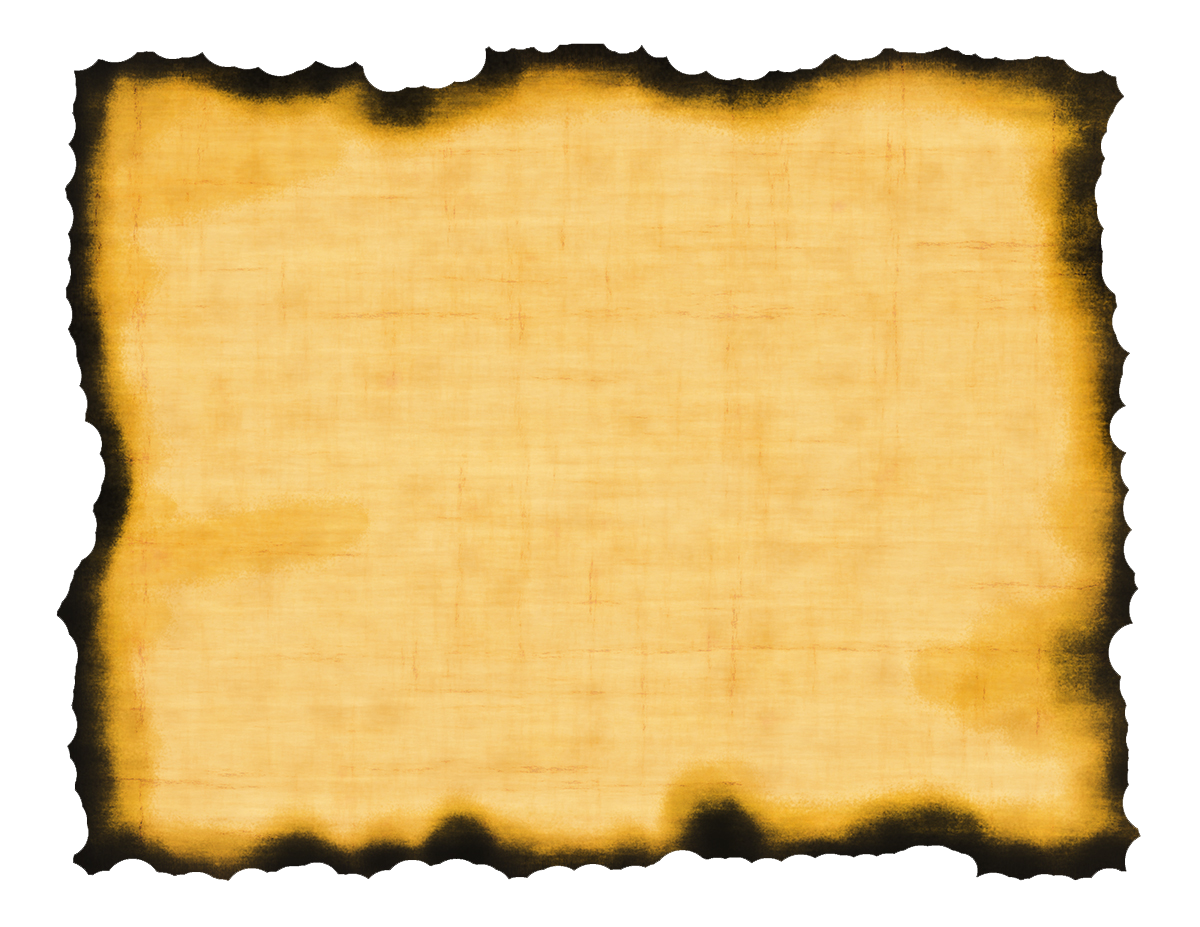
\includegraphics[width=480bp]{papiro.png}};
    \node at (0,3.5) [rectangle]{\parbox{350bp}{
      \begin{center}
        {\Huge\bfseries  内容简要}
        \end{center}
      {\Large\bfseries
        这部分我整理了在绘图学习中一些~Tikz 绘图的笔记,部分图是学习手册上的、部分是自己绘制的、也有自己搜集的其他人绘制的图,这些图主要的特点就是在生活工作尤其是教育教学,科研学术上用到,具体的内容包括:}
        {\bfseries
        \begin{enumerate}[label=\arabic*.,topsep=.5em]
            \setlength\parskip{.1em}
            \setlength{\baselineskip}{10pt}
            \item TikZ/PGFplots 曲线图绘制
            \item TikZ/PGFplots 柱状图/立体图绘制
            \item TikZ/PGFplots + Animate 动图绘制案例收集
            \item Pgfplots 学术绘图
            \end{enumerate}}

            \vfill
                      图片来源:https://codeload.github.com/livro-aberto/fracoes\_livro\_piloto/zip/master
                      }

                 };

                \end{tikzpicture}

\vfill
\dotfill~~\href{http://www.latexstudio.net.}{\textcolor{cyan}{LaTeX 工作室}}

\clearpage
 \section{TikZ/PGFplots 曲线的绘制}
 \thispagestyle{empty}
 \subsection{一般函数曲线的绘制}

 曲线的绘制,我认为能够根据函数表达式,在确定好自变量区间,然后选择适当的坐标轴比例,就可以绘制是最方便的,毕竟不需要描点连线等繁琐的步骤,至于对绘图最后装饰则需要根据你自己的需要即可,根据函数表达式绘图,我们给出一些案例:

 \textbf{多项式函数的绘制}

 \begin{lstlisting}[gobble=8]
          %  \definecolor{myback}{RGB}{53,64,89}
          %  \definecolor{mycolor}{RGB}{51,51,51}
          %  \definecolor{Orange}{RGB}{102,51,0}
          %  \definecolor{Green}{RGB}{0,102,51}
          %  \definecolor{Blue}{RGB}{15,107,108}
          %  \definecolor{Yellow}{RGB}{153,151,51}
        \begin{tikzpicture}[yscale=0.5]
          \draw[->,Orange](-0.5,0)--(5,0);
          \draw[->,Orange](0,-1)--(0,8);
          \draw[color=red, thick, domain=0:5,smooth,samples=100] plot ({\x},{\x}) node[right] {\tiny\(f(x)=x\)};
          \draw[color=blue,thick,domain=0:4,smooth,samples=100] plot ({\x},{\x^(3/2)}) node[right] {\tiny\(f(x)=x^\frac{3}{2}\)};
          \draw[color=cyan, thick, domain=0:2.7,smooth, samples=100] plot ({\x},{\x^(2)}) node[right] {\tiny\(f(x)=x^2\)};
          \draw[color=green,thick,domain=0:2.2,smooth,samples=100]plot({\x},{\x^(5/2)}) node[below] {\tiny\(f(x)=x^\frac{5}{2}\)};
          \draw[color=violet, thick, domain=0:2,smooth, samples=100] plot ({\x},{\x^(3)}) node[right] {\tiny\(f(x)=x^3\)};
          \draw[color=orange, thick, domain=0:1.7,smooth, samples=100] plot ({\x},{\x^(4)}) node[left] {\tiny\(f(x)=x^4\)};
          \draw[color=Green, thick, domain=0:1.5,smooth, samples=100] plot ({\x},{\x^(5)}) node[left] {\tiny\(f(x)=x^5\)};
          \draw[color=Blue, thick, domain=0:1.35,smooth, samples=100] plot ({\x},{\x^(6)}) node[left] {\tiny\(f(x)=x^6\)};
          \draw[color=yellow,thick,domain=0:5,smooth, samples=100] plot ({\x},{\x^(1/3)}) node[above] {\tiny\(f(x)=\sqrt[3]{x}\)};
          \draw[color=pink, thick,domain=0:5,smooth,samples=100] plot ({\x},{\x^(2/3)}) node[above] {\tiny\(f(x)=\sqrt[3]{x^2}\)};
          \draw[color=purple,thick,domain=0:5,smooth,samples=600] plot ({\x},{\x^(1/4)}) node[below] {\tiny\(f(x)=\sqrt[4]{x}\)};
          % 右边三个函数图像的绘制
          \draw[color=red, thick, domain=-1:3,smooth, samples=100] plot ({\x},{(1/10)*\x^(3)-2*\x^(2)+4*\x+4}) node[right] {\tiny\(f(x)=\frac{1}{10}x^3-2x^2+4x+4\)};
          \draw[color=blue, thick, domain=-1:2.6,smooth, samples=100] plot ({\x},{e^((2/3)*\x)}) node[right] {\tiny\(f(x)=e^\frac{3}{2}x\)};
          \draw[color=Green, thick, domain=-1:4,smooth, samples=100] plot ({\x},{(1/4)*\x^(4)-2*\x^(3)+(11/2)*\x^2-6*\x+2}) node[above] {\tiny\(f(x)=\frac{1}{4}x^4-2x^3+4x+\frac{11}{s}-6x+2\)};
          \draw[color=cyan,thick,domain=-1:5,smooth,samples=100] plot ({\x},{e^(-\x)}) node[below] {\tiny\(f(x)=\frac{1}{e^x}\)};
        \end{tikzpicture}
 \end{lstlisting}

 \vspace{3pt}
 \hfil\begin{minipage}[c]{0.51\textwidth}
  \begin{tikzpicture}[scale=0.6]
    \draw[draw=Blue,dashed,fill=cyan!15!white](-6,-4) rectangle (6,4);
    \node[scale=1] at (-0.5,0) {
      \begin{tikzpicture}[yscale=0.5]
        \draw[->,Orange](-0.5,0)--(5,0);
  \draw[->,Orange](0,-1)--(0,8);
  \draw[color=red, thick, domain=0:5,smooth, samples=100]
        plot ({\x},{\x}) node[right] {\tiny\(f(x)=x\)};
  \draw[color=blue, thick, domain=0:4,smooth, samples=100]
        plot ({\x},{\x^(3/2)}) node[right] {\tiny\(f(x)=x^\frac{3}{2}\)};
  \draw[color=cyan, thick, domain=0:2.7,smooth, samples=100]
        plot ({\x},{\x^(2)}) node[right] {\tiny\(f(x)=x^2\)};
  \draw[color=green, thick, domain=0:2.2,smooth, samples=100]
        plot ({\x},{\x^(5/2)}) node[below] {\tiny\(f(x)=x^\frac{5}{2}\)};
  \draw[color=violet, thick, domain=0:2,smooth, samples=100]
        plot ({\x},{\x^(3)}) node[right] {\tiny\(f(x)=x^3\)};
  \draw[color=orange, thick, domain=0:1.7,smooth, samples=100]
        plot ({\x},{\x^(4)}) node[left] {\tiny\(f(x)=x^4\)};
  \draw[color=Green, thick, domain=0:1.5,smooth, samples=100]
        plot ({\x},{\x^(5)}) node[left] {\tiny\(f(x)=x^5\)};
  \draw[color=Blue, thick, domain=0:1.35,smooth, samples=100]
        plot ({\x},{\x^(6)}) node[left] {\tiny\(f(x)=x^6\)};
  \draw[color=yellow, thick, domain=0:5,smooth, samples=100]
        plot ({\x},{\x^(1/3)}) node[above] {\tiny\(f(x)=\sqrt[3]{x}\)};
  \draw[color=pink, thick, domain=0:5,smooth, samples=100]
        plot ({\x},{\x^(2/3)}) node[above] {\tiny\(f(x)=\sqrt[3]{x^2}\)};
  \draw[color=purple!20!red, thick, domain=0:5,smooth, samples=600]
        plot ({\x},{\x^(1/4)}) node[below] {\tiny\(f(x)=\sqrt[4]{x}\)};
   \end{tikzpicture}
    };

  \end{tikzpicture}
  \vspace{2pt}
\end{minipage}
\quad
\begin{minipage}[c]{0.45\textwidth}
  \centering
  \vspace{3pt}
  \begin{tikzpicture}[scale=0.6]
 % \draw[Orange](-6.5,-4)--(-6.5,4);
  \draw[draw=Blue,dashed,fill=cyan!15!white](-6,-4) rectangle (6,4);
  \node[scale=1] at (0.5,0) {
    \begin{tikzpicture}[yscale=0.5]
      \draw[->,Orange](-0.5,0)--(5,0);
\draw[->,Orange](0,-1)--(0,8);
\draw[color=red, thick, domain=-1:3,smooth, samples=100]
      plot ({\x},{(1/10)*\x^(3)-2*\x^(2)+4*\x+4}) node[right] {\tiny\(f(x)=\frac{1}{10}x^3-2x^2+4x+4\)};
\draw[color=blue, thick, domain=-1:2.6,smooth, samples=100]
      plot ({\x},{e^((2/3)*\x)}) node[right] {\tiny\(f(x)=e^\frac{3}{2}x\)};
\draw[color=Green, thick, domain=-1:4,smooth, samples=100]
      plot ({\x},{(1/4)*\x^(4)-2*\x^(3)+(11/2)*\x^2-6*\x+2}) node[above] {\tiny\(f(x)=\frac{1}{4}x^4-2x^3+4x+\frac{11}{s}-6x+2\)};
 \draw[color=cyan, thick, domain=-1:5,smooth, samples=100]
      plot ({\x},{e^(-\x)}) node[below] {\tiny\(f(x)=\frac{1}{e^x}\)};
 \end{tikzpicture}
  };

\end{tikzpicture}
\vspace{2pt}
\end{minipage}

\textbf{三角函数图像的绘制}

三角函数基本绘图命令:

\begin{lstlisting}[gobble=8]
        \begin{tikzpicture}[yscale=0.5]
        \draw[->,Orange](-4,0)--(4,0);
        \draw[->,Orange](0,-4)--(0,4);
        \draw[color=red, thick, domain=-pi:pi,smooth, samples=200] plot ({\x},{(sin(\x r))^2}) node[above right] {\(g\left(x\right)=\sin^2 x\)};
        \draw[color=cyan, thick, domain=-pi:pi,smooth, samples=200] plot ({\x},{(cos(\x r))^2}) node[above right] {\(g\left(x\right)=\cos^2 x\)};
        \draw[color=blue, thick, domain=-pi:(2/3)*pi,smooth, samples=200] plot ({\x},{(2*sin(2*\x r))}) node[above right] {\(g\left(x\right)=2\sin 2 x\)};
        \draw[color=green, thick, domain=-pi:(1/2)*pi,smooth, samples=200] plot ({\x},{(3*cos(4*\x r))}) node[above right] {\(g\left(x\right)=3\cos 4 x\)};
        \draw[color=gray, thick, domain=-(1/4)*pi:(1/4)*pi,smooth, samples=200] plot ({\x},{(tan(\x r))}) node[above right] {\(g\left(x\right)=3\cos 4 x\)};
        \end{tikzpicture}
\end{lstlisting}

\vspace{3pt}
\begin{minipage}[c]{0.51\textwidth}
  \centering
  \begin{lstlisting}[gobble=8]
        \begin{tikzpicture}
         \foreach \i in {0,0.02,...,2} % foreach 循环语句
           \draw
                [
                 draw=cyan,  % 绘制线条颜色
                 rotate=-124 % 旋转角度
                ]
                ($(0,0) !1! \i*180:(3,2)$)--($(0,0) !1! \i*620:(3,2)$);
                % 在圆上标记100个等分点,依次从0标记到99,每个点连接标记是它3倍
                %的点,最后形成心线!
        \end{tikzpicture}
  \end{lstlisting}
  \vspace{2pt}
\end{minipage}
\hfil
\begin{minipage}[c]{0.45\textwidth}
  \centering
  \vspace{3pt}
  \begin{tikzpicture}[scale=0.6]
     \draw[Orange,dashed](-6.5,-4)--(-6.5,4);
     \draw[draw=Blue,dashed,fill=cyan!15!white](-6,-4) rectangle (6,4);
     \node[scale=1] at (0,0) {
       \begin{tikzpicture}[yscale=0.5]
         \draw[->,Orange](-4,0)--(4,0);
   \draw[->,Orange](0,-4)--(0,4);
   \draw[color=red, thick, domain=-pi:pi,smooth, samples=200] plot ({\x},{(sin(\x r))^2}) node[above right] {\(g\left(x\right)=\sin^2 x\)};
   \draw[color=cyan, thick, domain=-pi:pi,smooth, samples=200] plot ({\x},{(cos(\x r))^2}) node[above right] {\(g\left(x\right)=\cos^2 x\)};
   \draw[color=blue, thick, domain=-pi:(2/3)*pi,smooth, samples=200] plot ({\x},{(2*sin(2*\x r))}) node[above right] {\(g\left(x\right)=2\sin 2 x\)};
   \draw[color=green, thick, domain=-pi:(1/2)*pi,smooth, samples=200] plot ({\x},{(3*cos(4*\x r))}) node[above right] {\(g\left(x\right)=3\cos 4 x\)};
  %  \draw[color=gray, thick, domain=-(1/4)*pi:(1/4)*pi,smooth, samples=200] plot ({\x},{(tan(\x r))}) node[above right] {\(g\left(x\right)=3\cos 4 x\)};
    \end{tikzpicture}
     };

   \end{tikzpicture}
\vspace{2pt}
\end{minipage}
\thispagestyle{empty}
\begin{center}
  \begin{tikzpicture}[scale=1]
    \draw[draw=Blue,dashed,fill=cyan!15!white](-6,-4) rectangle (6,4);
    \node[scale=1] at (0,0) {
      \begin{tikzpicture}[yscale=0.025]
        \draw[->,Orange](-6,0)--(6,0);
        \draw[->,Orange](0,-100)--(0,100);
   \draw[color=blue, thick, domain=-pi:pi,smooth, samples=200] plot ({\x},{(tan(\x r))})
   node[above right] {\(g\left(x\right)=\tan x\)};
   \draw[color=cyan, thick, domain=-pi:pi,smooth, samples=600] plot ({\x},{((1/8)*tan(20*\x r))})
   node[below right] {\(g\left(x\right)=\frac{1}{8}\tan 20x\)};

% \draw[color=gray, thick, domain=-1:1,smooth, samples=200,yscale=40] plot ({\x},{(rad(asin(\x)))}) node[above right] {\(g\left(x\right)=3\cos 4 x\)};
%  \draw[color=gray, thick, domain=-(1/4)*pi:(1/4)*pi,smooth, samples=200] plot ({\x},{(tan(\x r))}) node[above right] {\(g\left(x\right)=3\cos 4 x\)};
% \draw[color=gray, thick, domain=-(1/4)*pi:(1/4)*pi,smooth, samples=200] plot ({\x},{(tan(\x r))}) node[above right] {\(g\left(x\right)=3\cos 4 x\)};
   \end{tikzpicture}
    };
    \node[scale=1] at (5.5,3) {\begin{minipage}{0.4\textwidth}
      \begin{lstlisting}[gobble=8]
        \draw[color=cyan, thick, domain=-pi:pi,smooth,
         samples=600] plot ({\x},{((1/8)*tan(20*\x r))})
      node[below right] {\(g\left(x\right)=\frac{1}{8}\tan 20x\)};
      \end{lstlisting}
    \end{minipage}
    };

    \node[scale=1] at (-4,3) {\begin{minipage}{0.4\textwidth}
      \begin{lstlisting}[gobble=8]
        \draw[color=blue, thick, domain=-pi:pi,smooth,
         samples=200] plot ({\x},{(tan(\x r))})
        node[above right] {\(g\left(x\right)=\tan x\)};
      \end{lstlisting}
    \end{minipage}
    };
  \end{tikzpicture}
\end{center}


\begin{minipage}[c]{0.51\textwidth}
  \centering
  \begin{lstlisting}[gobble=8]
    \begin{tikzpicture}[yscale=0.5]
    \draw[color=red, thick, domain=-1:1,smooth, samples=200] plot ({\x},{(rad(sin(\x r)))}) node[above right] {\(g\left(x\right)=\text{arcsin}^2 x\)};
    \draw[color=cyan, thick, domain=-1:1,smooth, samples=200] plot ({\x},{rad(acos(\x r))}) node[above right] {\(g\left(x\right)=\text{arccos}^2 x\)};
    \draw[color=blue, thick, domain=-50:50,smooth, samples=200,xscale=0.1] plot ({\x},{rad(atan(\x r))}) node[above right] {\(g\left(x\right)=\text{arctan x}\)};
  \end{tikzpicture}
  \end{lstlisting}
  \vspace{2pt}
\end{minipage}
\hfil
\begin{minipage}[c]{0.45\textwidth}
  \centering
  \vspace{3pt}
  \begin{tikzpicture}[scale=0.6]
     \draw[Orange,dashed](-6.5,-4)--(-6.5,4);
     \draw[draw=Blue,dashed,fill=cyan!15!white](-6,-4) rectangle (6,4);
     \node[scale=1] at (0,0) {
       \begin{tikzpicture}[yscale=0.5]
         \draw[->,Orange](-4,0)--(4,0);
         \draw[dashed,green](-1,-4)--(-1,4);
         \draw[dashed,green](1,-4)--(1,4);
   \draw[->,Orange](0,-4)--(0,4);
   \draw[color=red, thick, domain=-1:1,smooth, samples=200] plot ({\x},{(rad(asin(\x)))}) node[above=0.2cm] {\(g\left(x\right)=\text{arcsin} x\)};
    \draw[color=cyan, thick, domain=-1:1,smooth, samples=200] plot ({\x},{(rad(acos(\x)))}) node[above right] {\(g\left(x\right)=\text{arccos}x\)};
    \draw[color=blue, thick, domain=-30:30,smooth, samples=600,xscale=0.1] plot ({\x},{rad(atan(\x))}) node[above right] {\(g\left(x\right)=\text{arctan x}\)};
    \end{tikzpicture}
     };

   \end{tikzpicture}
\vspace{2pt}
\end{minipage}

 \subsection{封闭曲线及参数表达式函数曲线的绘制}

\textbf{封闭曲线的绘制}

% \begin{lstlisting}[gobble=8]
%     \begin{tikzpicture}[yscale=0.5]
%     \draw[color=red, thick, domain=-1:1,smooth, samples=200] plot ({\x},{(rad(sin(\x r)))}) node[above right] {\(g\left(x\right)=\text{arcsin}^2 x\)};
%     \draw[color=cyan, thick, domain=-1:1,smooth, samples=200] plot ({\x},{rad(acos(\x r))}) node[above right] {\(g\left(x\right)=\text{arccos}^2 x\)};
%     \draw[color=blue, thick, domain=-50:50,smooth, samples=200,xscale=0.1] plot ({\x},{rad(atan(\x r))}) node[above right] {\(g\left(x\right)=\text{arctan x}\)};
%   \end{tikzpicture}
%   \end{lstlisting}



\thispagestyle{empty}
  \begin{tikzpicture}[scale=1]
    \draw[draw=Blue,dashed,fill=cyan!15!white](-6,-4) rectangle (6,4);
    \node[scale=1] at (0,0) {
      \begin{tikzpicture}
        \draw[->,Orange](-6,0)--(6,0);
        \draw[->,Orange](0,-3)--(0,3);
   \draw[color=blue, thick, domain=0:2*pi,smooth,samples=300, variable=\p]
            plot ({2*cos(\p r)},{2*sin(\p r)});
   \draw[color=cyan, thick, domain=0:2*pi,smooth,samples=300, variable=\p]
            plot ({3*cos(\p r)},{sin(\p r)});
 \draw[color=red, thick, domain=0:2*pi,
        smooth,samples=300, variable=\p]
            plot ({2*cos(\p r)+1},{sin(\p r)-1});
            \draw[color=yellow, thick, domain=0:2*pi,
        smooth,samples=300, variable=\p]
            plot ({cos(\p r)-2},{sin(\p r)-1});
   \end{tikzpicture}
    };
    \node[scale=1] at (5.5,3) {\begin{minipage}{0.4\textwidth}
      \begin{lstlisting}[gobble=8]
        \draw[color=blue, thick, domain=0:2*pi,
        smooth,samples=300, variable=\p]
            plot ({cos(\p r)},{sin(\p r)});
      \end{lstlisting}
    \end{minipage}
    };

    \node[scale=1] at (-4,3) {\begin{minipage}{0.4\textwidth}
      \begin{lstlisting}[gobble=8]
        \draw[color=cyan, thick, domain=0:2*pi,
        smooth,samples=300, variable=\p]
            plot ({3*cos(\p r)},{sin(\p r)});
      \end{lstlisting}
    \end{minipage}
    };

    \node[scale=1] at (4,-3) {\begin{minipage}{0.4\textwidth}
      \begin{lstlisting}[gobble=8]
        \draw[color=red, thick, domain=0:2*pi,
        smooth,samples=300, variable=\p]
            plot ({2*cos(\p r)+1},{sin(\p r)-1});
      \end{lstlisting}
    \end{minipage}
    };

    \node[scale=1] at (-4,-3) {\begin{minipage}{0.4\textwidth}
      \begin{lstlisting}[gobble=8]
        \draw[color=yellow, thick, domain=0:2*pi,
        smooth,samples=300, variable=\p]
            plot ({cos(\p r)-2},{sin(\p r)-1});
      \end{lstlisting}
    \end{minipage}
    };
  \end{tikzpicture}


\begin{tikzpicture}[scale=1]
    \draw[draw=Blue,dashed,fill=cyan!15!white](-6,-4) rectangle (6,4);
    \node[scale=1] at (0,0) {
      \begin{tikzpicture}
        \draw[->,Orange](-6,0)--(6,0);
        \draw[->,Orange](0,-3)--(0,3);
 \draw[color=red, thick, domain=-60:60,
        smooth,samples=300]
            plot ({2*sec(\x)},{tan(\x)});
 \draw[color=red, thick, domain=120:240,
        smooth,samples=300]
            plot ({2*sec(\x)},{tan(\x)});
 \draw[color=red, thick, domain=-60:60,
        smooth,samples=300]
            plot ({2*sec(\x)-2},{tan(\x)-1});
   \end{tikzpicture}
    };
    \node[scale=1] at (5.5,3) {\begin{minipage}{0.4\textwidth}
      \begin{lstlisting}[gobble=8]
        \draw[color=red, thick, domain=-60:60,
        smooth,samples=300]
            plot ({2*sec(\x)},{tan(\x)});
      \end{lstlisting}
    \end{minipage}
    };

    \node[scale=1] at (-4,3) {\begin{minipage}{0.4\textwidth}
      \begin{lstlisting}[gobble=8]
        \draw[color=red, thick, domain=120:240,
        smooth,samples=300]
            plot ({2*sec(\x)},{tan(\x)});
      \end{lstlisting}
    \end{minipage}
    };

    \node[scale=1] at (0,-3) {\begin{minipage}{0.4\textwidth}
      \begin{lstlisting}[gobble=8]
        \draw[color=red, thick, domain=-60:60,
        smooth,samples=300]
            plot ({2*sec(\x)-2},{tan(\x)-1});
      \end{lstlisting}
    \end{minipage}
    };


  \end{tikzpicture}


\noindent
  \begin{lstlisting}[gobble=8]
          \begin{tikzpicture}[yscale=0.5]
          \draw[->,Orange](-4,0)--(4,0);
          \draw[->,Orange](0,-4)--(0,4);
          \draw[color=red, thick, domain=0:360,smooth,samples=300, variable=\t]plot ({\t}:{3*abs(cos(2*\t))}) node[above right]{\(\rho=3|\cos\left(2\theta\right)|\)};
          \draw[color=cyan, thick, domain=0:360,smooth,samples=300, variable=\t]plot ({\t}:{4*abs((cos(8*\t))}) node[above=2cm]{\(\rho=4|\cos\left(8\theta\right)|\)};
          \draw[color=yellow, thick, domain=0:360,smooth,samples=300, variable=\t]plot ({\t}:{abs((cos(15*(\t)))-2}) node[right=1cm]{\(\rho=4|\cos\left(15\theta-2\right)|\)};
    \end{tikzpicture}
  \end{lstlisting}
  \vspace{2pt}
  \begin{tikzpicture}[scale=0.6]
     \draw[draw=Blue,dashed,fill=cyan!15!white](-8,-8) rectangle (20,8);
     \node[scale=1] at (0,0) {
       \begin{tikzpicture}
   \draw[color=red, thick, domain=0:360,smooth,samples=300, variable=\t]
            plot ({\t}:{3*abs((cos(2*\t))}) node[above right]{\(\rho=3|\cos\left(2\theta\right)|\)};
    \draw[color=cyan, thick, domain=0:360,smooth,samples=300, variable=\t]
            plot ({\t}:{4*abs((cos(8*\t))}) node[above=2cm]{\(\rho=4|\cos\left(8\theta\right)|\)};
    \end{tikzpicture}
     };

\node[scale=1] at (13,0) {
       \begin{tikzpicture}
   \draw[color=yellow, thick, domain=0:360,smooth,samples=300, variable=\t]
            plot ({\t}:{abs((cos(15*(\t)))-2}) node[right=1cm]{\(\rho=4|\cos\left(15\theta-2\right)|\)};
    \end{tikzpicture}
};

   \end{tikzpicture}
\thispagestyle{empty}
\begin{tikzpicture}[scale=0.6]
     \draw[draw=Blue,dashed,fill=cyan!15!white](-8,-8) rectangle (20,8);
     \node[scale=1] at (-3,0) {
       \begin{tikzpicture}
    \draw[color=cyan, thick, domain=0:360,smooth,samples=300, fill=pink,variable=\t]
            plot ({\t}:{3*abs((sin(15*\t))});
    \end{tikzpicture}
     };

\node[scale=1] at (11,0) {
       \begin{tikzpicture}
   \draw[color=red, thick, domain=0:360,smooth,samples=300, fill=yellow,variable=\t]
            plot ({\t}:{(2/3)*abs((sin(15*(\t)))-5}) node[right=1cm]{\(\rho=4|\sin\left(15\theta-4\right)|\)};
    \end{tikzpicture}
};

   \end{tikzpicture}
\thispagestyle{empty}


